\section{Modeling of the \Fermi bubbles at low latitudes}
\label{sec:Modeling}

\begin{comment}
One of the main problems in the analysis of the FB near the GC is the 
presence of the foreground emission components, 
such as the interactions of cosmic rays with the interstellar gas and radiation fields.
In order to test the possible effects of the foreground emission modeling,
we use several methods to estimate the contribution of the foreground emission to the data.

In particular, there is a tentative
displacement of the FB to the right of the GC, i.e., negative Galactic latitudes \citep{2016ApJS..223...26A, 2017ApJ...840...43A},
with a spectrum that is harder than the spectrum of the FB at high latitudes \citep{2017ApJ...840...43A}.
If we assume that the Galactic emission components are approximately symmetric with respect to the GC,
then we can simply mask PS and calculate the difference in gamma-ray flux to the left and to the right from the GC.
The difference should be approximately equal to the asymmetric part of the FB emission
under the assumption that the other Galactic components and unresolved PS are symmetric with respect to the GC
(Section \ref{sec:data_diff}).

In order to further test the hypothesis of the asymmetric and hard emission from the FB at low latitudes,
we use the data at energies $\lesssim \SI{1}{GeV}$ to create a template of the Galactic emission,
provided that the expected contribution of the FB at these energies is small relative to the rest of the Galactic components.
Then we fit the template derived from the low-energy data together with an isotropic template at higher energies
outside of the FB area.
The FB intensity is determined by extrapolating the model inside the FB area using the full template and by subtracting the model
from the data (Section \ref{sec:le_data_model}).
As an alternative approach, instead of fitting outside of the FB area, we add to the model independent flat rectangular templates with the size
approximately following the FB size and fit the model over the whole sky.
The flux attributed to these rectangular templates is used as an estimate of the average flux in the FB in the corresponding areas
(Section \ref{sec:box_model}).

We also calculate the flux attributed to the bubbles using one of the diffuse emission models from \citep{2017ApJ...840...43A}
(Section \ref{sec:galprop_model}).

\end{comment}

\subsection{West -- East asymmetry in the data}
\label{sec:data_diff}

As a first simple check of the asymmetry at low latitudes, we compare the \Fermi-LAT data east and west of the Galactic center. 
We mask the 200 brightest 3FGL Point sources (PS)  with a circle of radius $\frac{\delta}{\sqrt{2}} + 1^\circ$ where $\delta = 0\degr\!\!.46$ is the characteristic size of the pixels. We also symmetrize the PSs relative to the GC in order to avoid possible bias by masking more pixels on one side of the GC. 
This PS mask is also used in the following sections. 
The data is averaged over a region to the West (longitudes $0^\circ < \ell < 10^\circ$) and to the East ($-10^\circ < \ell  <  0^\circ$) of the Galactic center for different latitudes. The regions have a latitude width of $10^\circ$ for $b >|10^\circ|$ and a width of  $4^\circ$ for  $b <|10^\circ|$. 
The difference of the averaged intensity of emission West minus East of the GC is shown in Fig. \ref{fig:data_diff}. 
The error bars in show the statistical errors.
At high latitudes, $b >|10^\circ|$, the emission is relatively symmetric. 
The emission for latitudes $b \in (-6^\circ, -2^\circ)$ and $b \in (-2^\circ, 2^\circ)$ shows excess emission to the West of the Galactic center, which remains significant at high energies. 


\begin{figure}[h]
\centering
 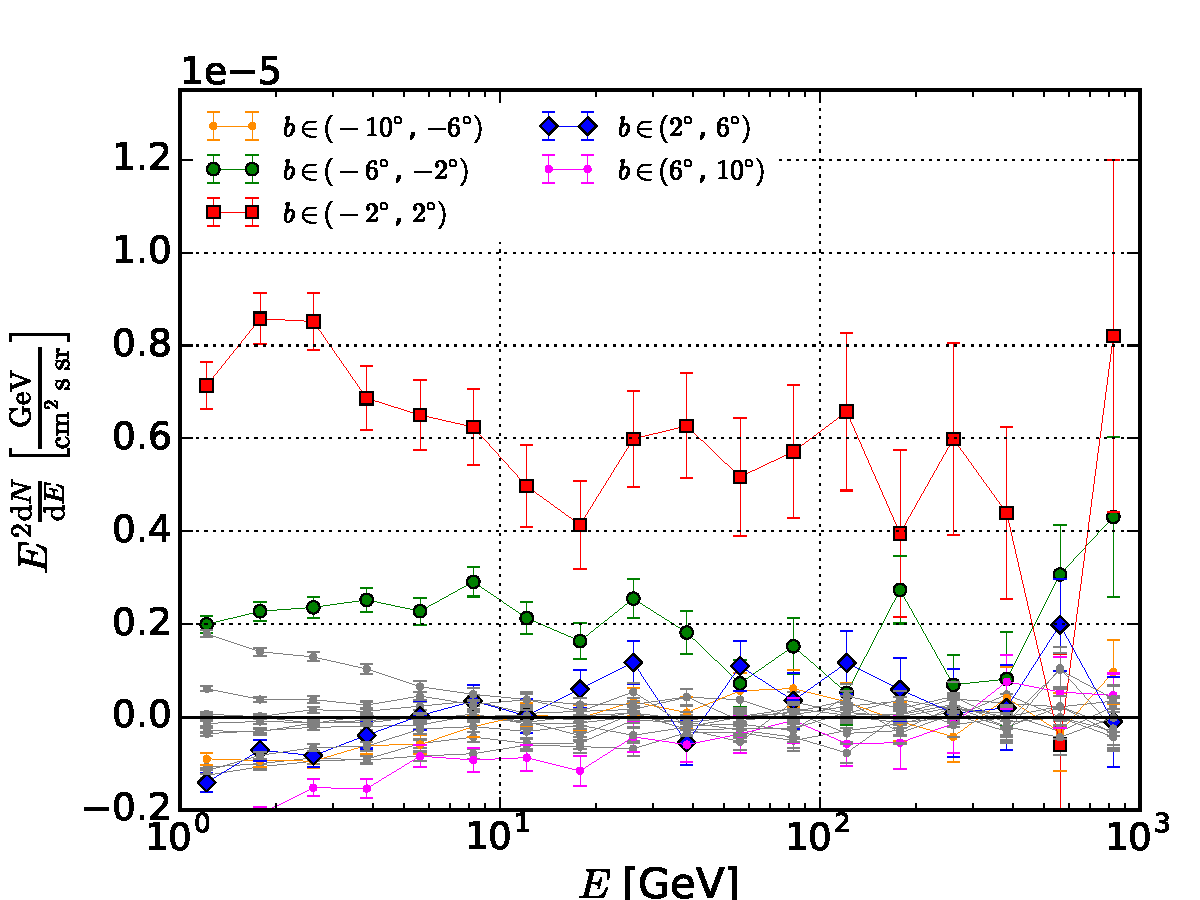
\includegraphics[width=0.5\textwidth]{plots/Difference_data_for_different_latitudes.pdf}
 \caption{Difference West minus East in the \Fermi-LAT intensity relative to the GC after masking bright PSs.
 The PS mask is made symmetric using point reflection relative to the GC.
 The West (East) region has $-10^\circ < \ell <0^\circ$ ($0^\circ < \ell <10^\circ$). }
 \label{fig:data_diff}
\end{figure}

\subsection{Low-energy data as a background model}
\label{sec:le_data_model}

\begin{figure*}[t]
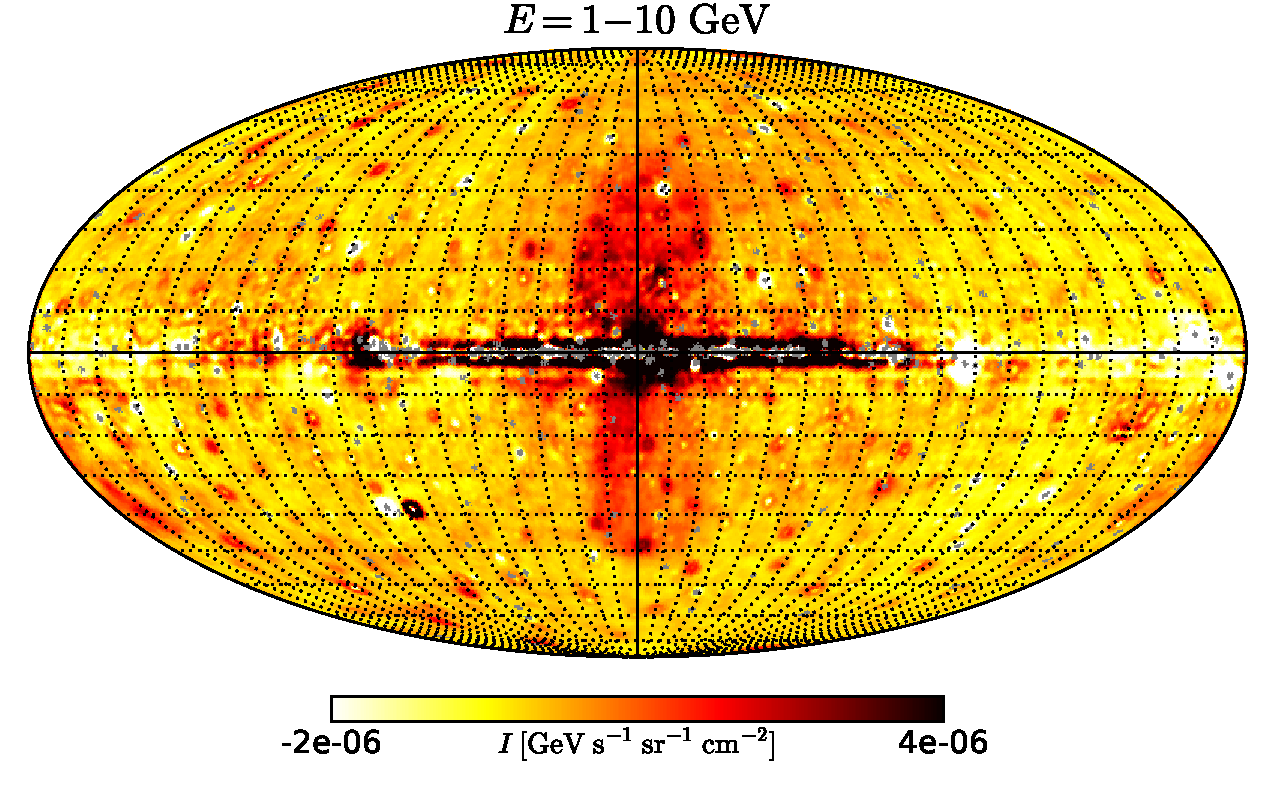
\includegraphics[width=0.33\textwidth]{plots/Mollweide_LowE_03-10GeV_flux_source_range_0.pdf}
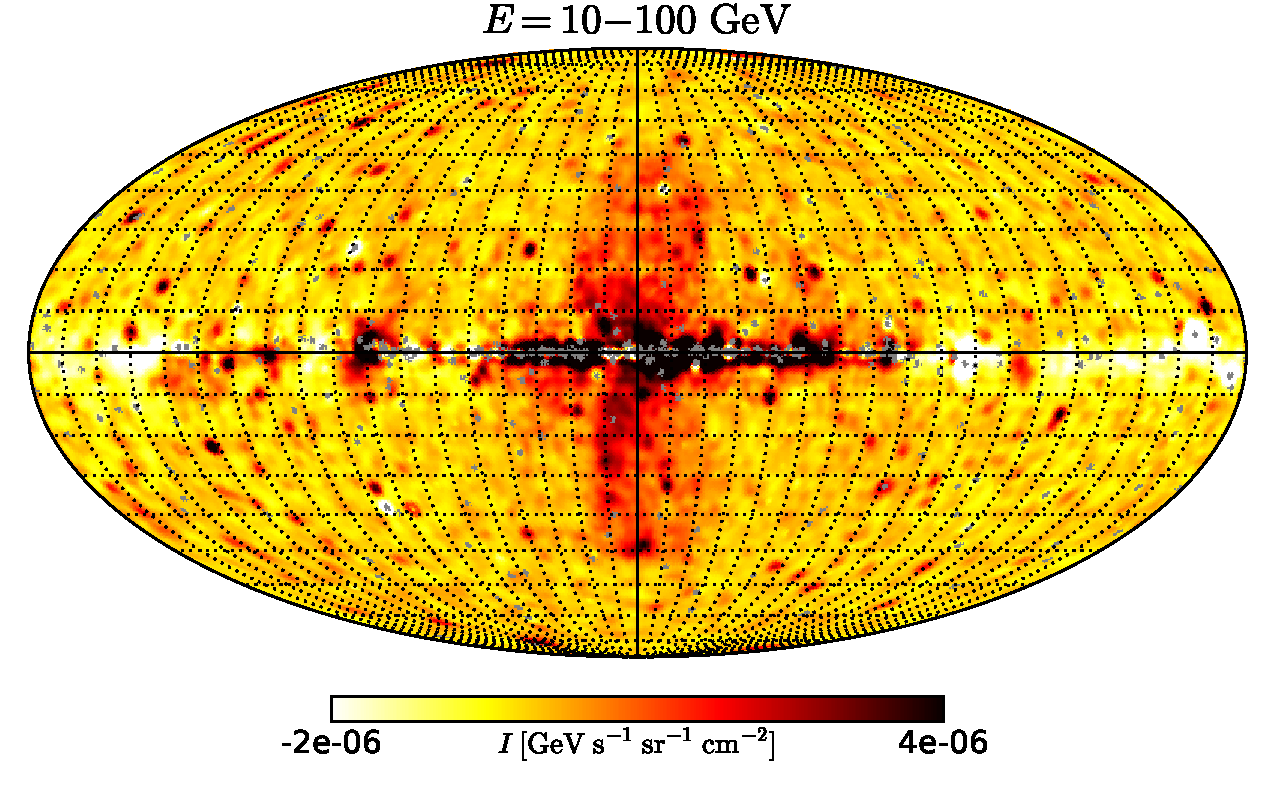
\includegraphics[width=0.33\textwidth]{plots/Mollweide_LowE_03-10GeV_flux_source_range_1.pdf}
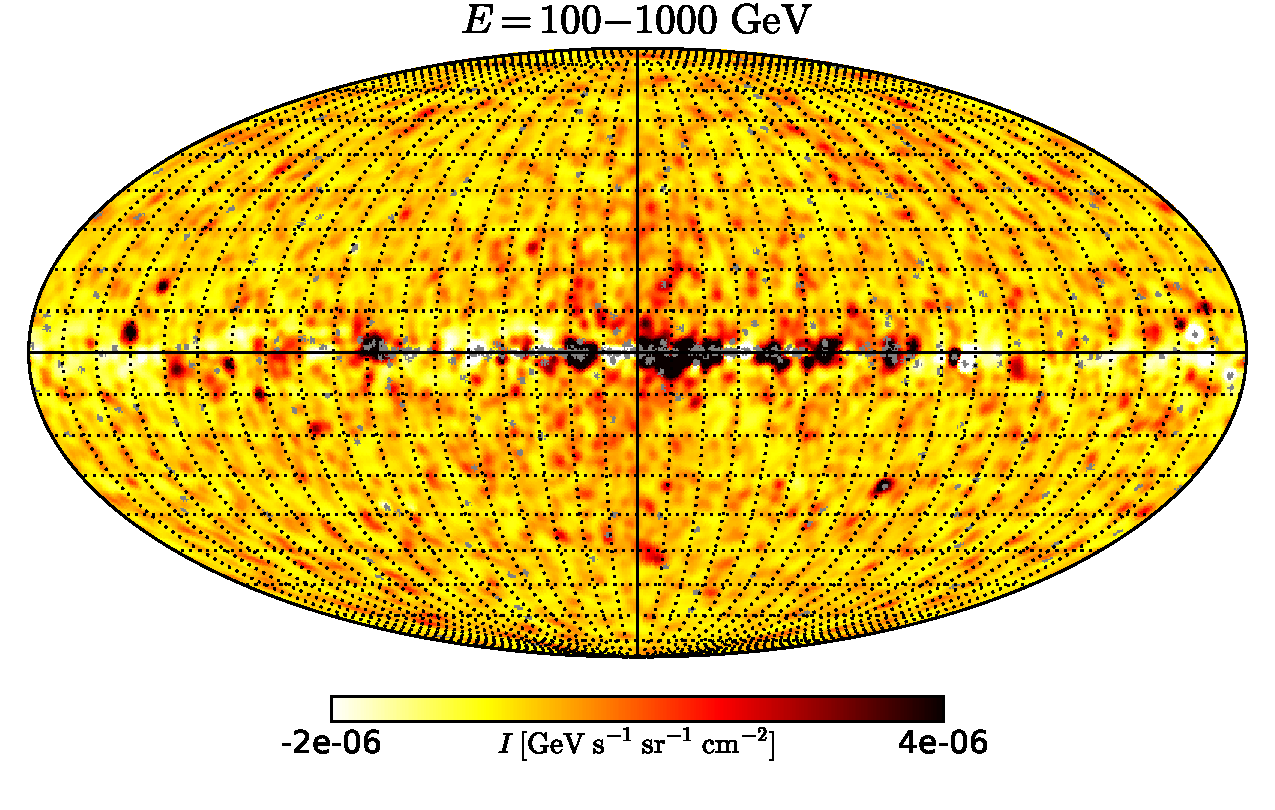
\includegraphics[width=0.33\textwidth]{plots/Mollweide_LowE_03-10GeV_flux_source_range_2.pdf}
\caption{Integrated SED intensity of the residuals of the low-energy model in three different energy ranges. }
\label{fig:Maps_lowE}
\end{figure*}

Gamma rays produced in interactions of CR with gas and IC scattering dominate the gamma-ray emission around the GC in the energy range $E \lesssim \SI{1}{GeV}$. 
Consequently, low-energy \Fermi-LAT data is a good tracer for diffuse gamma-ray emission in the Galactic plane and can be used to create a spatial template for the Galactic foreground.
The 68\% containment for the \Fermi-LAT photons between $\SI{316}{MeV}$ and $\SI{1}{GeV}$ (averaged with $E^{-2}$ spectrum) is about $1^\circ\!\!.5$,
which is much worse than the sub-degree angular resolution above $\SI{1}{GeV}$.
In order to compensate for the difference in the angular resolution, 
we smooth the data in each high-energy bin with a Gaussian kernel of $\ang{1}$ (which corresponds to $68\%$ containment angle of
$1^\circ\!\!.5$ in 2 dimensions).

We cut the sky horizontally in latitude stripes with the width of $\ang{4}$ and define our model in each stripe and energy bin separately. 
In the latitude stripe $\ell$ and energy bin $E$ our model consists of two terms:

\be
N^\model_{\ell}(E,x) = k_{\ell}(E) \cdot \tilde N^\low_{\ell}(E,x) + c_\ell(E) \cdot \tau(x,E),
\ee
where $k_{\ell}(E) \cdot \tilde N^\low_\ell(E, x)$ is proportional to the low-energy photon counts summed over 
$n_\low = 3$ energy bins between between $\SI{316}{MeV}$ and $\SI{1}{GeV}$ 
rescaled by the ratio of exposures at low and at high energies:
\be
\tilde N^\low_\ell(E,x) = \frac{1}{n_\low} \left(\sum_{\epsilon \in (0.3 - \SI{1.0}{GeV})} \frac{N^\low(\epsilon, x)}{\tau(\epsilon,x)}\right) \cdot \tau(E,x),
\ee
The term $c_\ell(E) \cdot \tau(x,E)$ is proportional to exposure $\tau(x,E)$, it accounts for the isotropic extragalactic background and partially compensates for the latitude dependent IC emission. 

We determine the parameters $c_{\ell}(E)$ and $k_{\ell}(E)$ by fitting the model to the \Fermi-LAT data in energy bins $E > \SI{1.0}{GeV}$
using Poisson likelihood (with Python iminuit minimizer). Since we smooth the data before the fit, the Poisson log-likelihood is an approximation in this case. 
In order to avoid an overcompensation of the \Fermi bubbles, the region $-20^\circ < \ell < 20^\circ$ is excluded from the fit. PSs are masked with the mask described in Section \ref{sec:data_diff}.

%\red{Dima: do we symmetrize the PS mask in the analysis as well, not only in the calculation of the asymmetry in the data?}

After we fit the model in each latitude stripe, we interpolate it inside the bubbles ROI and 
find the residual by subtracting the model from the data.
Figure \ref{fig:Maps_lowE} shows the residual SED intensity integrated for three different energy ranges%
\footnote{The integral of the SED intensity between $E_0$ and $E_1$ is defined as
$W = \int_{E_0}^{E_1} E \frac{dN}{dE} dE.$}.
The FB are clearly visible in the first two energy ranges, $E = 1 - \SI{10}{GeV}$ and $E = 10 - \SI{100}{GeV}$, for 
$E = \SI{100}{GeV} - \SI{1}{TeV}$ the statistics is low, but one can still see an excess near the GP.

\subsection{Rectangles model of the bubbles}
\label{sec:box_model}

In the previous subsection, we exclude the approximate ROI of the FB.
In this subsection, we perform the fit over the whole sky and model the emission from the FB by rectangles of small size.
%Our first simple ansatz for a model of the FB consists of rectangular templates that approximately cover the area of the FB. 
In order to explore the east-west asymmetry of the FB, 
we introduce two rectangular templates in each latitude stripe $\ell$ and energy bin $E$: 
one east ($-20^\circ - 0^\circ$) and one west ($0^\circ - 20^\circ$) of the GC.
We use the same foreground model as in Section \ref{sec:le_data_model} plus the isotropic template.
Overall, the model has four terms in each energy bin:

\be
\begin{split}
N^\model_{\ell}(E,x) &= k_{\ell}(E) \cdot \tilde N^\low_{\ell}(E,x) + c_\ell(E) \cdot \tau(x,E)\\
&\quad + R^\east_\ell(E) + R^\west_\ell(E).
\end{split}
\ee
where the scaling parameters $k_{\ell}(E)$, $c_{\ell}(E)$, $R^\east_\ell(E)$, and $R^\west_\ell(E)$ are determined independently 
in each $4^\circ$ latitude stripe and in each energy bin $E > \SI{1.0}{GeV}$
by  fitting the model to the \Fermi-LAT data.
The map of residuals plus the rectangles model integrated for $E = 10 - \SI{100}{GeV}$ is shown in Fig. \ref{fig:Maps_Rectangles}.
%Here we plot the sum of the residual and the rectangles model.
%With residual we denote the sum of the rectangles-model residual and the rectangles template in the following.

\begin{figure}[h]
\centering
 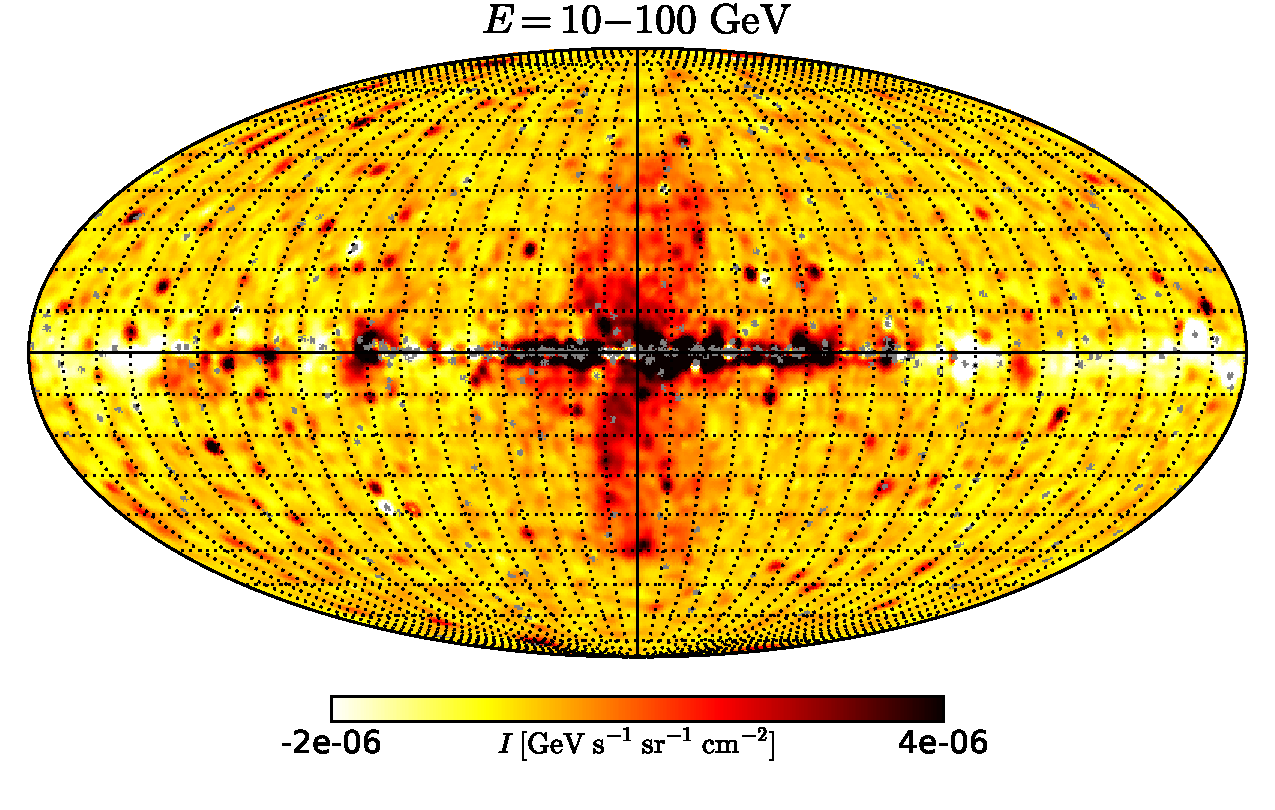
\includegraphics[width=0.5\textwidth]{plots/Mollweide_Boxes_residual+boxes_03-10GeV_flux_source_range_1.pdf}
 \caption{Integrated SED intensity of the residuals plus the rectangles model of the FB derived in Section \ref{sec:box_model}.}
 \label{fig:Maps_Rectangles}
\end{figure}


\subsection{GALPROP model of the foreground and PS refitting}
\label{sec:galprop_model}


\begin{figure}[h]
\centering
 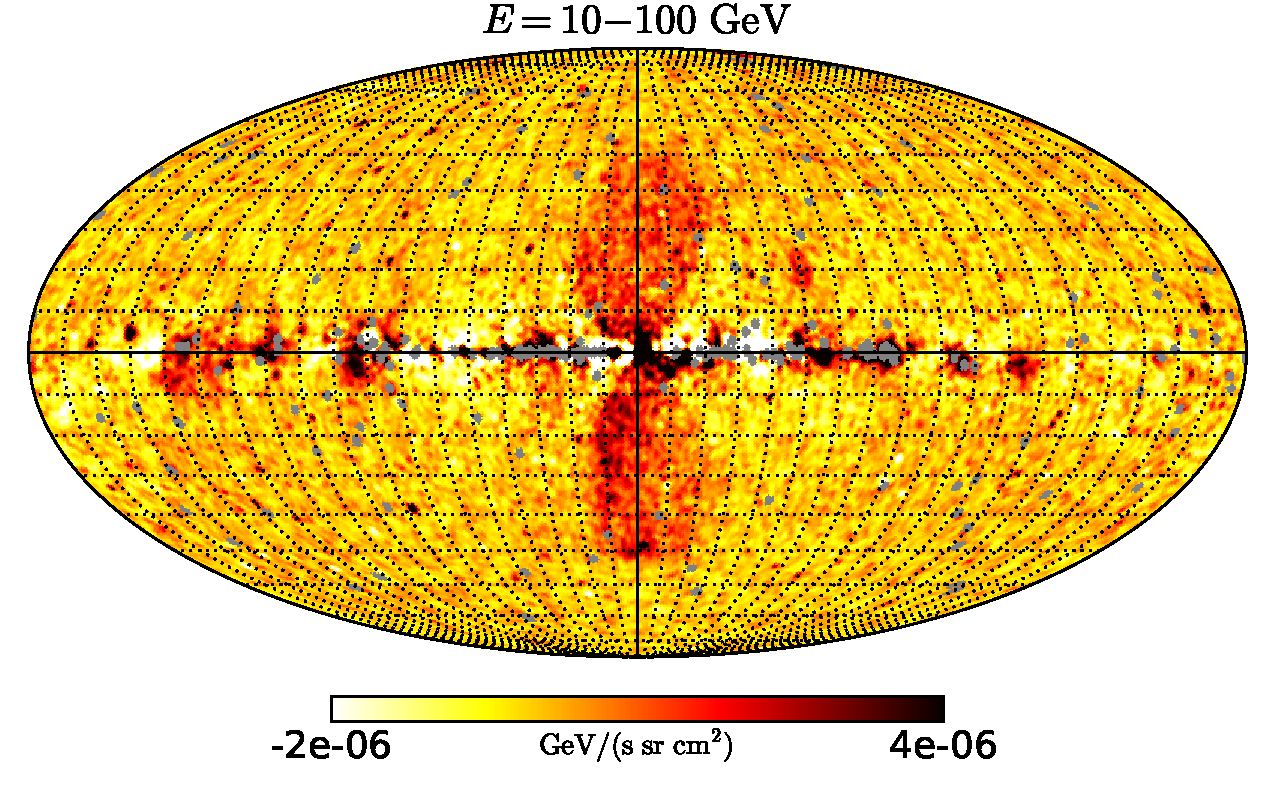
\includegraphics[width=0.5\textwidth]{plots/Mollweide_GALPROP_source_range2.pdf}
 \caption{Integrated SED intensity of the residuals in the GALPROP model.}
 \label{fig:Maps_GALPROP}
\end{figure}

In this section we fit the gamma-ray data using a model derived with the GALPROP
galactic propagation code v54.1
\citep{Moskalenko:1997gh, Strong:1998fr, Strong:2004de, Ptuskin:2005ax, 2007ARNPS..57..285S, Porter:2008ve,Vladimirov:2010aq}\footnote{\url{http://galprop.stanford.edu}}. 
The model for the diffuse components is the same as the Sample model in \cite{2017ApJ...840...43A}.
The difference is that, within $10^\circ$ from the GC, we do not mask PS and refit 40 PS with largest 
flux between 10 and 100 GeV.

We use GALPROP to calculate templates for the Galactic diffuse emission components.
In particular, in each energy bin we determine 5 templates for gamma rays produced in 
interactions of hadronic CR with gas and bremsstrahlung in 5 Galactocentric rings: 
0 -- 1.5\,kpc, 1.5 -- 3.5\,kpc, and 3.5 -- 8\,kpc; 8 -- 10\,kpc, and 10 -- 50\,kpc. 
We use 3 inverse Compton templates corresponding to the three interstellar radiation fields: CMB, 
infrared emission, and starlight.
In addition to GALPROP templates, we use a flat template for the \Fermi bubbles at latitudes $|b| > 10^\circ$~\citep{2014ApJ...793...64A}. 
In the Sample Model we account for Loop~I using a geometric model \citep[e.g., Figure 2 of][]{2014ApJ...793...64A}
based on a polarization survey at 1.4 GHz~\citep{Wolleben:2007pq}.
The Sun \citep{2007Ap&SS.309..359O, 2006ApJ...652L..65M, 2008A&A...480..847O, 2013arXiv1307.0197J} and the Moon templates are obtained with the \Fermi Science Tools%
\footnote{\url{http://fermi.gsfc.nasa.gov/ssc/data/analysis/scitools/solar_template.html}}.
We also include a generalized Navarro-Frenk-White (gNFW) profile with index $\gamma = 1.25$ and scaling radius $r_{\rm s} = 20\;{\rm kpc}$.


For the PS, we add sources in the 3FGL catalog~\citep{2015ApJS..218...23A} to form a template
in each energy bin.
We create independent templates for the Large Magellanic cloud and the Cygnus region.
The remaining extended sources are also added in a separate template.
We mask 200 brightest sources outside $R = 10^\circ$ from the GC and include independent templates
for 40 sources with largest flux between 10 and 100 GeV within $10^\circ$ from the GC.
In Figure \ref{fig:Maps_GALPROP} we show the residual emission plus the \Fermi bubbles model and the gNFW model summed over energies between 10 and 100 GeV.



